% =====================================================================
% III. Methodology: dataset construction (subsections A to G).
% Fragment without \section; followed by sections/methodology_models.tex (H to J).
% Heading levels: \section -> III.  \subsection -> A.  \subsubsection -> 1)
% =====================================================================
\providecommand{\arch}[1]{\path{#1}}

This section describes, in order, how the original public dataset was turned into the 35,007 region-of-interest (ROI) images used to train and compare the four models (Sections~\ref{sec:models} and \ref{sec:protocol}). Fig.~\ref{fig:pipeline} summarizes the pipeline and the number of items at each stage. All figures come from files versioned in the project repository.

% ---------------------------------------------------------------------
\subsection{Data Source}
\label{sec:origin}
The \emph{Lumbar Spine MRI Dataset} (Mendeley Data) \cite{sudirman2019} was used. It contains studies from 515 patients with symptomatic low back pain and 48,345 MRI slices, and it has already been used in previous work on disc herniation classification \cite{sari2025} and on Pfirrmann grading of degeneration \cite{natalia2024}. The studies were acquired on a single scanner, a 1.5~T Siemens MAGNETOM Essenza, and are distributed as DICOM files with the \arch{.IMA} extension, in one folder per patient. Folders are numbered 0001 to 0575; the 60 missing numbers are already missing at the source. Slices have a pixel size of 0.729~mm, a thickness of 4~mm and a center-to-center spacing of 4.8~mm. The \texttt{.IMA} files keep their DICOM metadata, but the \texttt{PatientID} field is empty throughout the corpus and the source only keeps study and series identifiers. Therefore, in this work each folder is treated as one patient: the 515 folders correspond to the 515 patients, and every mention of ``patient'', including the patient-level split, refers to the folder.

Of the 515 patients, 414 kept usable slices after cleaning (Section~\ref{sec:cleaning}) and 399 after the ROI quality exclusions (Section~\ref{sec:roi}). Each of the 414 folders corresponds to a different \texttt{StudyInstanceUID} and no \texttt{StudyTime} is repeated; there is no evidence of duplicated patients, although, with the identifier empty, this cannot be fully ruled out.

\begin{figure}[!htb]
\centering
\begin{tikzpicture}[
  box/.style={draw, rounded corners=2pt, align=left, text width=0.56\columnwidth, inner sep=2pt, font=\scriptsize},
  num/.style={align=left, text width=0.34\columnwidth, font=\scriptsize\bfseries},
  arrow/.style={-{Stealth[length=1.5mm]}, thick},
  node distance=3mm]
  \node[box] (a) {1. Public dataset (Mendeley), \texttt{.IMA} files};
  \node[num, right=2mm of a] {515 patients, 48,345 slices};
  \node[box, below=of a] (b) {2. Filtering by series name (sagittal T2)};
  \node[num, right=2mm of b] {8,794 slices};
  \node[box, below=of b] (c) {3. Central 40\%, DICOM$\to$PNG and manual cleaning};
  \node[num, right=2mm of c] {1,086 slices, 414 patients};
  \node[box, below=of c] (d) {4. L1--S1 crop and disc detection (128$\times$128 ROI)};
  \node[num, right=2mm of d] {5,385 ROIs};
  \node[box, below=of d] (e) {5. Pre-labeling, human review and exclusions};
  \node[num, right=2mm of e] {5,123 ROIs, 399 patients};
  \node[box, below=of e] (f) {6. Patient-level split 70/15/15};
  \node[num, right=2mm of f] {279 / 60 / 60 patients};
  \node[box, below=of f] (g) {7. Augmentation within each partition};
  \node[num, right=2mm of g] {35,007 images};
  \foreach \i/\j in {a/b,b/c,c/d,d/e,e/f,f/g} \draw[arrow] (\i) -- (\j);
\end{tikzpicture}
\caption{Dataset preparation pipeline and number of items at each stage.}
\label{fig:pipeline}
\end{figure}

% ---------------------------------------------------------------------
\subsection{Source Cleaning}
\label{sec:cleaning}
Each patient has several series, and only some of them are useful for this problem. Table~\ref{tab:discarded} lists what was discarded and why.

\begin{table}[!htb]
\centering\footnotesize
\caption{Series discarded from each study and reason}
\label{tab:discarded}
\begin{tabular}{>{\raggedright\arraybackslash}p{0.33\columnwidth}>{\raggedright\arraybackslash}p{0.58\columnwidth}}
\toprule
Series & Reason for discarding \\
\midrule
\arch{LOCALIZER_0001} & Very low-resolution localizers used to position the patient; they provide no anatomical or texture information. \\
\arch{POSDISP_[4]_T2_TSE_TRA_...} & Sagittal views with overlaid lines that mark the axial planes and distort the texture. \\
\arch{T1_TSE_SAG_...}, \arch{T1_TSE_TRA_...} & On T1, fat is bright and fluid is dark: disc hydration, the basis of the Pfirrmann scale \cite{pfirrmann2001}, cannot be assessed, and mixing T1 and T2 alters brightness ranges. \\
\arch{T2_TSE_TRA_...} (axial) & Axial slices in batches of 3 to 5 per level; they would need to be matched to each disc. Left for a future phase. \\
\arch{T2_TIRM_SAG_...} & Fat-suppressed inversion recovery, with a contrast different from T2 TSE. Removed during manual cleaning. \\
\bottomrule
\end{tabular}
\end{table}

The process had four steps, each with its own script (folder \arch{scripts/preprocesamiento/}); Table~\ref{tab:stages} gives the number of slices and patients after each one.
\begin{enumerate}
  \item \arch{ingestion.py} copies the files whose name contains ``T2'' and ``SAG'', except localizers and \arch{POSDISP}. This criterion let through, in addition to the sagittal T2 TSE series, the sagittal T2 TIRM series of 44 patients.
  \item \arch{limpiar_slices.py} keeps the central 40\% of each patient's slices (it drops the first and last 30\%, sorted by file name), where the spinal canal and the L1--S1 region are visible.
  \item \arch{convertidor_dcm_a_png.py} converts to 8-bit PNG with a single scale per series: the 1st and 99.5th percentiles computed over tissue pixels. Neither CLAHE nor any other enhancement was applied, so as not to alter the relative T2 signal on which the diagnostic criterion relies; the way intensity is normalized affects the performance of deep learning on MRI, at least in segmentation \cite{jimenezpartinen2026}, so a single per-series normalization was kept across the whole corpus.
  \item Manual cleaning of the PNGs: cervical or knee studies, dark or artifact-laden sagittal T2 slices, and all TIRM slices were removed.
\end{enumerate}

\begin{table}[!htb]
\centering\footnotesize
\caption{Slices (per sequence) and patients after each cleaning step}
\label{tab:stages}
\begin{tabular}{lrrrr}
\toprule
Step & TSE & TIRM & Total & Patients \\
\midrule
Original corpus & -- & -- & 48,345 & 515 \\
Name filtering & 8,094 & 700 & 8,794 & 515 \\
Central 40\% & 3,235 & 284 & 3,519 & 515 \\
Manual cleaning & 1,086 & 0 & 1,086 & 414 \\
\bottomrule
\end{tabular}
\end{table}

After cleaning, \textbf{1,086 sagittal T2 TSE slices from 414 patients} remained (2.6 slices per patient on average; between 1 and 6).

\subsubsection{Slice Selection Error}
While reviewing traceability, once the dataset had been built, an error was found in step~2. For the 44 patients with a TIRM series, the central 40\% was computed over the joint list of both series sorted by name. Because TIRM files sort before TSE files, the retained window covered the central TIRM slices and the first TSE slices (slices 1 to 6 of 15), which are lateral. The TIRM slices were removed during manual cleaning and, in 36 of those 44 patients, no usable TSE slice remained: they are 36 of the 101 patients lost between 515 and 414. The other 8 entered with slice 006 of 15, which is parasagittal rather than mid-sagittal. No TIRM slice reached the final dataset. Filtering only the \arch{T2_TSE_SAG} series and choosing the mid-sagittal slice within it, as other work on this corpus does \cite{natalia2024}, would have kept those patients. Due to time constraints the process was not redone, and the error is declared as a limitation. In addition, 17 patients have 30 TSE slices (possibly two series) and could be affected by the same computation; this was not verified.

% ---------------------------------------------------------------------
\subsection{Lumbar Region and Per-Disc ROI Cropping}
\label{sec:roi}
\subsubsection{L1--S1 Crop}
With \arch{aplicar_recortes.py}, each slice was cropped vertically to cover mainly L1--S1, replicating earlier manual crops by template matching (median matching score of 0.9996; only slice 0547\_008 fell below 0.99). The crop was extended by 60~px upwards and downwards up to the image border; this reduced the padding needed at L1-L2 from 779 of 1,080 crops (72\%) to zero.

\subsubsection{Disc Detector}
Detecting discs before classifying them is a common step in the literature, including the YOLO family on sagittal slices \cite{tan2024,sayed2025scirep}. To locate them, a detector was trained on an in-house Roboflow dataset (project \emph{Intervertebral Disks}, version~1): 100 slices (70 for training, 20 for validation and 10 for testing), with auto-orientation and resizing to 640$\times$640 with black borders, and no augmentation in Roboflow. The detector's five classes are the levels L1-L2 to L5-S1. A YOLOv8n box detector was fine-tuned. The model that generated the ROIs was trained for 100 epochs; a 200-epoch version was discarded because, on inspection, it detected discs where there were none. The detector only locates the disc level; it does not classify pathology.

Although Roboflow applied no augmentation, Ultralytics applies online augmentation by default during training (mosaic, scale, translation, color jitter and horizontal flip with probability 0.5). Flipping does not change a disc's level, because the L1-L2 to L5-S1 order is vertical; in the augmentation of the classification dataset, however, flipping was excluded (Section~\ref{sec:augmentation}).

The notebook used to train the deployed model did not save its metrics. To report performance, training was repeated with the same data and architecture (50 epochs, patience 30, batch 16, 640~px images, seed 42 and the same default augmentation; best validation epoch: 49). Table~\ref{tab:detector} summarizes that re-run at the operating threshold (confidence 0.35).

\begin{table*}[t]
\centering\footnotesize
\caption{Performance of the detector training re-run (run \texttt{detector\_discos\_v1\_s42}), used as an estimate of the model that generated the ROIs}
\label{tab:detector}
\begin{tabular}{lrrrrrrr}
\toprule
Partition & Slices & Precision & Recall & mAP50 & mAP50-95 & Slices with 5 levels & Mean IoU \\
\midrule
Validation & 20 & 0.922 & 0.964 & 0.962 & 0.663 & 95\% & 0.819 \\
Test       & 10 & 0.983 & 0.994 & 0.995 & 0.691 & 100\% & 0.843 \\
\bottomrule
\end{tabular}
\end{table*}

The hardest level is L1-L2 (on validation: precision 0.839, recall 0.820 and IoU 0.74); the other levels have a recall of 1.0. With only 20 and 10 slices, a single slice shifts the figures by several percentage points; it is a single run with a single seed, and the epoch was chosen on validation, so its figures are somewhat inflated. Moreover, they describe the re-run and not the deployed model, although both share data and architecture and differ only in the number of epochs.

\subsubsection{ROI Extraction}
With \arch{autocrop_rois.py}, detection runs on the crop and the patch is extracted from the full PNG by adding the offset. The box is enlarged (posterior margin 0.40, anterior 0.10 and vertical 0.50), made square and saved at 128$\times$128~px, one per level. Each crop is logged in \arch{roi_log.csv} with its box, center ordinate, confidence and padding per side. The result was \textbf{5,385 ROIs}. An anterior L5-S1 margin of 0.20 was tested against 0.10 and the gain was marginal, so 0.10 was kept. Fig.~\ref{fig:rois} shows the five ROIs of one slice.

\begin{figure*}[t]
\centering
\includegraphics[width=0.85\textwidth]{rois_0188_008.png}
\caption{The five original ROIs (L1-L2 to L5-S1) of slice 008 of patient 0188, as stored in the dataset (128$\times$128~px).}
\label{fig:rois}
\end{figure*}

\subsubsection{Quality Exclusions}
Objective rules were applied on \arch{roi_log.csv} (function \arch{elegibles()} in \arch{scripts/build_dataset.py}): a whole slice is discarded if any level is missing, if two adjacent levels overlap (IoU $>0.5$) or if the vertical order of the centers does not increase from L1-L2 to L5-S1; in addition, patient 0456, slice 0547\_008 and ROIs with detector confidence below 0.5 are excluded. In total, \textbf{262 ROIs} were excluded, affecting 48 patients; 15 patients were removed entirely. Thus, the 5,385 labeled ROIs become \textbf{5,123 ROIs from 399 patients}. Of the excluded ROIs, 207 were Protrusion, 38 Normal and 17 Degeneration.

% ---------------------------------------------------------------------
\subsection{Annotation and Relabeling}
\label{sec:annotation}
\subsubsection{Classes}
The annotation guide (\arch{docs/guias/guia_anotacion_4_clases.md}) defines four nominal classes: Normal, Degeneration, Bulge and Herniation. Degeneration was defined as loss of disc T2 signal or height without protrusion, in line with the Pfirrmann scale \cite{pfirrmann2001}. When several classes co-occur, the priority Herniation $>$ Bulge $>$ Degeneration $>$ Normal is applied; it only breaks labeling ties and is not a severity order. The guide gathers commonly used criteria and has not been validated by a radiologist. Labels were assigned by students, without a radiologist.

\subsubsection{Merging into Three Classes}
In the first run of the seed classifier, with the four classes (60 validation images), accuracy was 0.65 (95\% CI: 0.52--0.76), and 10 of the 21 errors were Herniation--Bulge confusions. Without an axial slice, the extent of the displaced material around the disc circumference, which is what separates the two entities in the consensus nomenclature \cite{fardon2014}, cannot be measured. Even with a standardized nomenclature, inter-radiologist agreement on disc contour is only fair to moderate \cite{arana2011}, and in computed tomography bulge and protrusion have been reported as the most confused pair of classes \cite{gao2025}. Herniation and Bulge were therefore merged into \textbf{Protrusion}, leaving three classes: Normal, Disc Degeneration and Protrusion. The merge is a post hoc decision, made after seeing the data, and is declared as such.

\subsubsection{Pre-Labeling and Review}
Labeling 5,385 ROIs from scratch was not feasible within the deadline, so a pre-labeling scheme with human review was followed, related to active learning \cite{wang2024al} and to iterative annotation in which a model proposes and a person corrects \cite{vandergraaf2024}. First, a balanced seed of about 300 ROIs was labeled by hand in Roboflow with the four original classes: 240 for training (60 per class) and 60 for validation (15 per class). Roboflow resized the images to 224$\times$224 and generated three outputs per training image (rotation of $\pm 5^{\circ}$ and brightness of $\pm 15\%$). The labels were refined over three versions, as morphological criteria were sharpened and the classes were reduced to three; some images were removed in the last one. Version~3, used for pre-labeling, has 719 training images (already augmented) and 84 validation images (24 Degeneration, 30 Normal and 30 Protrusion). A small YOLOv8s-cls classifier was trained on it (224$\times$224 input, up to 60 epochs, patience 15, batch 32, seed 42). On validation it reached an accuracy of 0.833 (95\% CI: 0.739--0.898) and an F1 of 0.784 for Degeneration, 0.852 for Normal and 0.857 for Protrusion; with only 84 validation images, these figures are a guide rather than a guarantee. The pre-labeler was an internal tool: it is none of the four compared models, and its only role was to speed up and organize the review.

The model pre-labeled the 5,385 ROIs with a class and a confidence (mean 0.946; median 1.0) and flagged 2,265 (42.1\%) for priority review. Protrusion predictions were always sent to review (2,039, of which 1,881 for that reason alone), because the initial sample of 70 ROIs suggested it was a minority class and the model, trained on balanced classes, was expected to over-predict it. The other 226 were flagged for confidence below 0.7, alone or together with a margin below 0.2 between the top two classes. The review showed the opposite: the model under-predicted Protrusion.

Afterwards, all ROIs, flagged or not, went through human review in two groups, A and B, of 2,693 and 2,692 ROIs, respectively. The final class is always the human decision. Of the 5,385 ROIs, 3,366 (62.5\%) kept the model's class and \textbf{2,019 (37.5\%) were corrected}. Table~\ref{tab:relabel} shows how the dataset was reorganized.

\begin{table}[!htb]
\centering\footnotesize
\setlength{\tabcolsep}{3.5pt}
\caption{Class proposed by the pre-labeler versus final class after human review (5,385 ROIs)}
\label{tab:relabel}
\begin{tabular}{lrrrrr}
\toprule
 & \multicolumn{3}{c}{Final class} & & \\
\cmidrule(lr){2-4}
Predicted & Normal & Degen. & Protr. & Total & Corrected \\
\midrule
Normal       & 1,086 & 32  & 1,387 & 2,505 & 56.6\% \\
Degeneration & 51    & 256 & 534   & 841   & 69.6\% \\
Protrusion   & 6     & 9   & 2,024 & 2,039 & 0.7\% \\
\midrule
Final total  & 1,143 & 297 & 3,945 & 5,385 & 37.5\% \\
\bottomrule
\end{tabular}
\end{table}

Of the 3,945 final Protrusion ROIs, 1,921 (48.7\%) arrived as Normal or Degeneration, whereas almost nothing the model predicted as Protrusion changed (15 of 2,039). Human review, not the model, set the class distribution of the dataset, and that distribution is highly imbalanced (Section~\ref{sec:balance}).

\subsubsection{Label Reliability}
Each ROI was reviewed by a single person (A or B); 408 of the 414 patients have ROIs reviewed by both, but no ROI was double-labeled. Consequently, \textbf{inter-annotator kappa cannot be computed}. Differences in criteria are nonetheless visible: A labeled Degeneration in 6.9\% of their ROIs and B in 4.1\%, and A corrected 35.3\% versus 39.7\% for B. It is not possible to separate how much of that difference is criterion and how much is sample composition. Non-expert labels introduce noise that reduces the generalization ability of networks \cite{shi2024}. In addition, since reviewers saw the model's suggestion, anchoring bias is possible: in radiology, incorrect AI advice has been observed to drag down physicians' diagnoses \cite{prinster2024}.

% ---------------------------------------------------------------------
\subsection{Patient-Level Split}
\label{sec:split}
Each patient contributes about 13 ROIs (5,123/399) from nearly identical neighboring slices. If the split were done by image, a patient would be spread across training and test, and the model could recognize the patient instead of the pathology, inflating the metrics (data leakage) \cite{brunekreef2024,rumala2023}. Therefore, \textbf{each patient goes entirely to a single partition}.

The split is 70/15/15 by patient, with seed 42. The script tries 20,000 random splits and keeps the one that best preserves, across the three partitions, the proportion of each class (triple weight) and of each level. Three partitions were used because validation serves to make decisions (epoch, hyperparameters, thresholds) and the test set to measure once at the end, with everything already decided. Table~\ref{tab:split} shows the result. The intersection of patients between partitions is empty and is checked with assertions in the script. Patients with at least one Degeneration ROI number 81, 17 and 22 in training, validation and test.

\begin{table}[!htb]
\centering\footnotesize
\setlength{\tabcolsep}{3.5pt}
\caption{Patient-level split and original ROIs per class}
\label{tab:split}
\begin{tabular}{lrrrrrr}
\toprule
Partition & Patients & Normal & Degen. & Protr. & ROIs & \% ROIs \\
\midrule
Training   & 279 & 771   & 194 & 2,612 & 3,577 & 69.8 \\
Validation & 60  & 170   & 44  & 564   & 778   & 15.2 \\
Test       & 60  & 164   & 42  & 562   & 768   & 15.0 \\
\midrule
Total      & 399 & 1,105 & 280 & 3,738 & 5,123 & 100 \\
\bottomrule
\end{tabular}
\end{table}

% ---------------------------------------------------------------------
\subsection{Data Augmentation}
\label{sec:augmentation}
To obtain more than 35,000 images with the same count per class in each partition from 5,123 original ROIs, data augmentation was used. Augmentation was always performed \emph{after} splitting and \emph{within} each partition, so that no copy crosses partitions: resampling before splitting biases metrics upwards \cite{demircioglu2024}. The number of copies per ROI is computed so that each class reaches the same target per partition: 8,167 images per class in training and 1,751 in validation and test, i.e., 35,007 in total (Table~\ref{tab:35k} and Fig.~\ref{fig:balancechart}).

\begin{table*}[t]
\centering\footnotesize
\caption{Final images per partition and class (same number per class in each partition), original ROIs and images per original}
\label{tab:35k}
\begin{tabular}{llrrrr}
\toprule
Partition & Class & Originals & Augmented & Total & Images per original \\
\midrule
Training   & Normal       & 771   & 7,396 & 8,167 & 10.6 \\
           & Degeneration & 194   & 7,973 & 8,167 & 42.1 \\
           & Protrusion   & 2,612 & 5,555 & 8,167 & 3.1  \\
Validation & Normal       & 170   & 1,581 & 1,751 & 10.3 \\
           & Degeneration & 44    & 1,707 & 1,751 & 39.8 \\
           & Protrusion   & 564   & 1,187 & 1,751 & 3.1  \\
Test       & Normal       & 164   & 1,587 & 1,751 & 10.7 \\
           & Degeneration & 42    & 1,709 & 1,751 & 41.7 \\
           & Protrusion   & 562   & 1,189 & 1,751 & 3.1  \\
\midrule
Total      &              & 5,123 & 29,884 & 35,007 & \\
\bottomrule
\end{tabular}
\end{table*}

\subsubsection{Transformations}
Mild geometric and photometric transformations, common in medical imaging \cite{islam2024}, were used: rotation of $\pm 8^{\circ}$, shift of up to $\pm 8\%$ of the size, zoom between 0.90 and 1.10, and brightness and contrast of $\pm 10\%$, with reflection padding at the borders. No flips (the anterior--posterior axis has anatomical meaning), elastic deformation or enhancement were used. Each copy is generated with a seed derived from a hash (SHA-256) of the ROI name, the global seed and the copy index, so the process is deterministic and reproducible.

\begin{figure}[!htb]
\centering
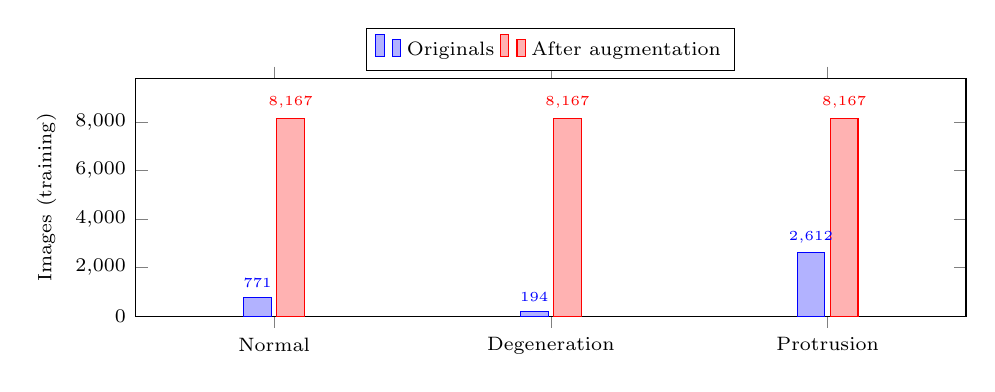
\begin{tikzpicture}
\begin{axis}[
  ybar, bar width=10pt, width=\columnwidth, height=4.6cm,
  symbolic x coords={Normal,Degeneration,Protrusion}, xtick=data,
  ymin=0, ymax=9800, ylabel={Images (training)},
  enlarge x limits=0.25, legend style={at={(0.5,1.03)},anchor=south,legend columns=2,font=\scriptsize},
  nodes near coords, every node near coord/.append style={font=\tiny},
  tick label style={font=\scriptsize}, ylabel style={font=\scriptsize}]
\addplot coordinates {(Normal,771) (Degeneration,194) (Protrusion,2612)};
\addplot coordinates {(Normal,8167) (Degeneration,8167) (Protrusion,8167)};
\legend{Originals, After augmentation}
\end{axis}
\end{tikzpicture}
\caption{Count-based balance in training: original ROIs and total after augmentation.}
\label{fig:balancechart}
\end{figure}

\subsubsection{Traceability}
Each file is named \arch{T2_TSE_SAG__0188_008_L4-L5__orig.png} (original) or \arch{..._aug012.png} (copy), with patient, slice and level. The manifest \arch{manifest_35k.csv} records, for each of the 35,007 images, its partition, class, patient, level, original ROI, reviewer and, for copies, the exact parameters (seed, angle, zoom, shifts, contrast and brightness); \arch{split_pacientes.csv} stores each patient's partition. The images are not uploaded to the repository: they are distributed as a 405~MB archive, and the repository keeps the manifests and the scripts that reproduce them from the public data.

\subsubsection{Checks}
The script verifies that (i) the patient sets of the three partitions are disjoint, (ii) every copy is in the same partition as its original, (iii) file names are unique, (iv) every PNG is intact, and (v) the total exceeds 35,000. The copies respect the declared ranges (angle between $-8^{\circ}$ and $8^{\circ}$, zoom and contrast between 0.90 and 1.10).

% ---------------------------------------------------------------------
\subsection{Class Balance and Level Bias}
\label{sec:balance}
The 1/3 balance per class is \emph{by count}, not by originals. Among the 5,123 original ROIs, Protrusion accounts for 73.0\% (3,738), Normal for 21.6\% (1,105) and Degeneration for 5.5\% (280); a classifier that always predicted Protrusion would be right about 73\% of the time. Copies equalize each class's contribution to training, but they add no new anatomy: the effective dataset size is the number of patients (399), and Degeneration, repeated about 42 times, has only 42 originals in the test partition, which leaves a wide margin of error on its recall. So that metrics are not inflated by near-identical copies, the main results are computed on the \textbf{originals} of the test partition, and the full set is reported separately. In addition, a model trained with a uniform prior tends to over-predict rare classes in the real population.

Table~\ref{tab:level} shows a strong bias: almost all pathology is concentrated at L4-L5 and L5-S1. A classifier that merely guessed the most frequent class at each level would get 3,842 of 5,123 ROIs right (75.0\%), so the level could act as a shortcut; shortcut learning makes measured performance overestimate real performance \cite{onglt2024}. Results are therefore also reported per level. This puts any accuracy threshold into perspective: a 95\% measured on these labels measures agreement with student labels and may be reached partly through the shortcut, and high internal figures tend to drop on external data \cite{yi2023}. For this reason, accuracy is accompanied by macro F1 and per-class recall: with imbalanced classes, the usual metrics are dominated by the majority class \cite{mosquera2024}.

\begin{table}[!htb]
\centering\footnotesize
\setlength{\tabcolsep}{4pt}
\caption{Eligible original ROIs by level and class}
\label{tab:level}
\begin{tabular}{lrrrrr}
\toprule
Level & Normal & Degen. & Protr. & Total & \% Protr. \\
\midrule
L1-L2 & 505 & 121 & 401   & 1,027 & 39.0 \\
L2-L3 & 383 & 94  & 550   & 1,027 & 53.6 \\
L3-L4 & 172 & 44  & 811   & 1,027 & 79.0 \\
L4-L5 & 15  & 5   & 1,005 & 1,025 & 98.0 \\
L5-S1 & 30  & 16  & 971   & 1,017 & 95.5 \\
\bottomrule
\end{tabular}
\end{table}
